% This is a sample LaTeX input file.  (Version of 9 April 1986) 
% 
% A '%' character causes TeX to ignore all remaining text on the line, 
% and is used for comments like this one.

\documentclass{article}    % Specifies the document style.
\usepackage{graphicx}
\usepackage{alltt}
\title{Ontology Engineering \& Semantic Web \\ Project Report}  % Declares the document's title. 
\author{Panagiotis Chatzichristodoulou and Kirill Tumanov}    % Declares the author's name
\date{March 27, 2014}   % Deleting this command produces today's date.

%
\begin{document}           % End of preamble and beginning of text.
%
\maketitle                 % Produces the title.
%
\begin{abstract}
%
This work serves as a reference and a summary document for the designed Student Lifecycle Management (SLM) system ontology, based on the SAP AG framework. It gives an overall structure of the ontology and describes the main functions of student lifecycle it reflects. For better comprehension this description is coupled with following the built-it exemplar individuals. The paper ends with discussion on ontology limitations and possible future work.
%
\end{abstract}
%
% 
\section{Introduction}
%
Ontology engineering is a field that studies the methods and methodologies of building ontologies. From an Artificial Intelligence point of view, an ontology is defined as: ``explicit specification of conceptualization"~\cite{Gruber}, meaning that ontologies are formal representations of sets of concepts and the relations between them within a domain. It must be noted that even though ontologies are build to serve as formal representations of a certain problem, ontologies should be build as problem-independent as possible. Consequently, an ontology about a car of a certain brand must also be able to represent cars of other brands without any modifications. 
% 
\section{Implementation}
%
The domain of the ontology described in this paper is SLM, meaning that the ontology build creates a framework that describes the SLM system. Despite the fact that it was based on SAP-SLM~\cite{sap}, the ontology can be used to model the student life outside of the framework and be easily extended to show more specific situations.

The ontology of SLM system was designed according to the available SAP AG framework, shown in Fig.~\ref{SAP}. The implementation itself was done in Protege 4.3.0 software in the Web Ontology Language (OWL) format. HermiT 1.3.8 was used as a means of reasoning. 
\begin{figure}[htbp]
  \centering
    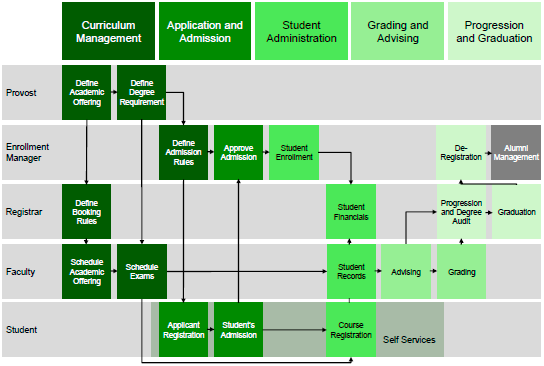
\includegraphics[width=0.8\textwidth]{Materials/Figures/1.png}
    \caption{SAP AG framework of SLM~\cite{sap}}
  \label{SAP}
\end{figure}

Although there is no clear specification of what procedures the system is able to reflect, it is relatively easy to understand what are the most essential ones. Some of the blocks shown here in the ontology were logically merged or united by their roles and underlying processes. E.g. ``Graduation" was merged with ``De-Registration" and has a lot in common with ``Define Degree Requirement". 

A more specific review of the ontology is done in the following subsections. They are organized on the built-in individuals, as a whole student lifecycle process.
%
\subsection{Application and Graduation}
%
Everything started when a British school graduate \textit{Bob Smith} heard from his friend \textit{Joey Miller} about the \textit{RWTH University}, who graduated on the same year. \textit{Joey} told him that some years ago he was a student at the \textit{Mathematics Department} of this university. He followed a \textit{Study Programme} in Mathematics very similar to the one in existence. Upon completion of the studies, he was awarded a \textit{BSc Degree} in Mathematics, de-registered by \textit{Sam Jones} - an \textit{Enrollment Manager} and included into the list of \textit{RWTH Alumni}. Now \textit{Joey} was going to attend an \textit{Alumni Meeting} organized by \textit{Terry Mitchel} - an \textit{Alumni Manager}.

\textit{Joey} inspired \textit{Bob} to take the same study programme as his, since \textit{Bob} was quite into Math. So, \textit{Bob} filed an \textit{Admission Request}, which includes all needed documents and side procedures, this request was received and fulfilled (processed) by the \textit{Enrollment Manager}. After the decision was made, the \textit{Admission Request} resulted in \textit{Admission Response}, which was sent back to \textit{Bob}. \textit{Bob} received the \textit{Response} and found himself accepted to the \textit{RWTH}. He later was enrolled as a \textit{Student} by the \textit{Enrollment Manager}. 
% 
\subsection{Study Programme}
%
\textit{Bob} being a Math \textit{Student} selected to pursue a \textit{Study Programme in Mathematics}, which culminates with an award of \textit{BSc Degree} to the graduates. The programme defined by \textit{Lilian Marshall} - a \textit{Provost}, apart from the rest includes \textit{Courses} in \textit{Linear Algebra} and \textit{Statistical Theory}. The programme and all its courses are taught in \textit{English}. In addition, the \textit{Study Programme} has a number of \textit{Specialization}s, among which are a \textit{Major in Mathematics} and a \textit{Minor in Statistics}.

\textit{Graduation Requirement}s for each \textit{Study Programme} are defined by the \textit{Provost}. These requirements mainly include the number of \textit{Credits} a \textit{Student} must obtain during the study. A certain amount of \textit{Credit}s is given for each \textit{Course}, while it also is awarded to a \textit{Student} upon a successful completion. A \textit{Course} in \textit{Statistical Theory} has a \textit{Linear Algebra} as a prerequisite. Each \textit{Course} is taught by a \textit{Faculty}. \textit{Course} is comprised of \textit{Lectures}.

Each \textit{Lecture} being an \textit{Event} has its \textit{Location}, start and end time, which are scheduled by \textit{Kyle Nillson} - a \textit{Scheduling Officer}. A \textit{Person} registered for the \textit{Course} the \textit{Lecture} is of may attend it. Each \textit{Lecture} may have a different teaching method: a lecture, a practical or a seminar.

A \textit{Course} may have one of the following statuses: booking, ended, fully booked or ongoing. When \textit{Course} is in a booking state, a \textit{Student} is able to, first, book a place in it and later to be registered. An end of a booking term is defined by the \textit{Course}'s booking deadline. Finally, after taking a \textit{Course} a \textit{Student} may fail it or complete successfully.

Successful completion or failure of a \textit{Course} is based on the \textit{Student}'s \textit{Grade} obtained at the corresponding \textit{Exam}. \textit{Exam} is an \textit{Event}, like a \textit{Lecture}, and thus has similar features. In addition, an \textit{Exam Paper} is issued for each \textit{Exam}, meaning a set of questions a \textit{Student} is to answer. A \textit{Faculty} member conducts an \textit{Exam}, grades the \textit{Exam Paper} and reports a \textit{Grade} to the \textit{Student}.

\textit{Bob}'s \textit{Linear Algebra} course is taught by \textit{Jeffry Hunt} - a \textit{Full Professor} of Mathematics, and a \textit{Statistical Theory} course by \textit{Samantha Kole} - a \textit{Senior Lecturer}. He is registered for both of them, and attends the first and second lectures of each one respectfully.
% 
\subsection{Student Administration}
%
A \textit{Student} being enrolled at a \textit{University} is obliged to pay \textit{Tuition}. This part of student finances a \textit{University} is concerned about. So since \textit{Bob} got enrolled he was a subject of tuition payment check. 

The check is a part of the \textit{Tuition Management} service of the \textit{University}. In \textit{RWTH} \textit{Student Administration Office} provides this \textit{Service}, with \textit{Frank de Boer} - a \textit{Registrar} being responsible for it. However, as \textit{Bob} just got accepted the first check was performed by the \textit{Enrollment Manager}, who filed the \textit{Tuition Fees Request} and sent it to \textit{Jessica Vervier} - a \textit{University Accountant}. She checked the \textit{RWTH} public account to see that the tuition fees were paid, thus fulfilling the \textit{Request}, which resulted in a positive \textit{Response} sent back to the \textit{Enrollment Manager}.

However not only finances but all the personal information and grades of a \textit{Student} are in the competence of the \textit{Student Administration Office}. This data is stored and retrieved from the \textit{RWTH} grade and personal info databases, accessible through a \textit{University Portal} in the Web. \textit{RWTH} \textit{Students} and \textit{University Personnel} have different privileges using the portal.
% 
\subsection{Advising}
%
Once \textit{Bob} became a \textit{Student} he started to take care of his upcoming \textit{Internship}. As he was new to the procedures he decided to ask an advise of the \textit{Mathematics Department} \textit{Study Advisor} - \textit{Gonny Millews}. To do so, \textit{Bob} filed a \textit{Request of Additional Info on the Internship} possibilities, which was a general e-mail on practice. \textit{Gonny} received his e-mail, thought of an answer and replied, providing him a general information an useful links. Therefore, she fulfilled the \textit{Request} and produced a \textit{Response} to it.

When \textit{Bob} received this information from the \textit{Study Advisor}, he contacted a company named \textit{Diamond LLC}. There he was said that they had a placement - an \textit{Internship} in Data Analysis. After thinking of his career prospects \textit{Bob} decided to accept the offer and fill the position. Since then, in addition to being a Mathematics \textit{Student} \textit{Bob} also plays a \textit{Role} of a \textit{Data Analyst}.
% 
\subsection{Visualization}
%
This section provides and analyses visualizations of the ontology. The visualizations provided are in the form of Cloud Views. Such views provide insight about the relations between its Terminology and Application. Firstly, in Fig.~\ref{classUsage} classes that are used the most in the ontology are displayed. That is the ones that have the most relations and provide the basis in which the ontology is build. As expected, the classes of \textit{Course}, \textit{Study Programme}, \textit{Student} and \textit{Role} play a major role in the ontology and serve as its backbone. On the other hand, classes like \textit{Database} and \textit{Document} are used much less even though they are essential to the structure of this ontology.

Secondly, information about the amount of functionality each individual within the ontology has is shown in Fig.~\ref{cloudIndi}. Again, instances of type \textit{Course}, \textit{Role}, \textit{Study Programme} and \textit{Student} are the most used ones. Furthermore instances like \textit{University Accountant} have much less connections despite being essential to the ontology. That is expected since some individuals provide the core of the ontology and are used more than others. That displays a good correlation between the Terminology of the ontology and its Application.
\begin{figure}[htbp]
  \centering
    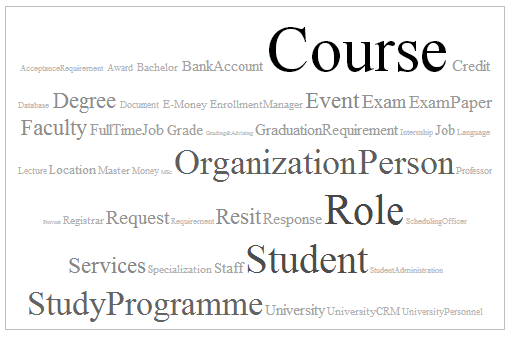
\includegraphics[width=0.8\textwidth]{Materials/Figures/classUsageCloud.png}
    \caption{Most used classes}
  \label{classUsage}
\end{figure}
\begin{figure}[htbp]
  \centering
    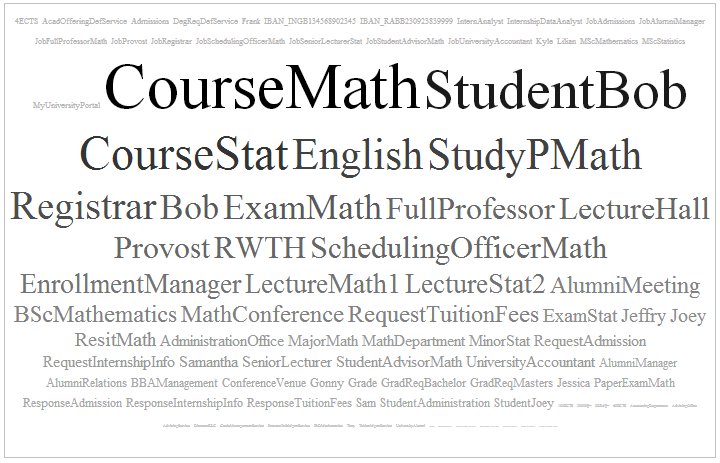
\includegraphics[width=0.8\textwidth]{Materials/Figures/cloudIndies.png}
    \caption{Most used individuals}
  \label{cloudIndi}
\end{figure}
% 
\subsection{Conclusion}
%
Building a proper ontology that is minimal and at the same time successfully represents a problem domain is not a trivial task. Major concern for a potential user of the ontology is the specifics of how certain relation chains where designed. Although it is a common concern of most ontologies, it should be considered its limitation. Future work should be focused on including missing or more detailed processes and relations, which will complete the SAP-SLM framework with new capabilities.
%
% ---- Bibliography ----
%
\begin{thebibliography}{99}
%
\bibitem {sap}
Solution in Detail: Higher Education and Research. Student Life Management.
SAP AG, \texttt{http://www.sap.com/bin/sapcom/en\_us/downloadasset.2013-12-dec\newline-11-11.higher-education-and-research-student-lifecycle-\newline management-pdf.html}(2013)

\bibitem{protege}
Protege ontology creation tool Website.\\
\texttt{http://protege.stanford.edu/}

\bibitem{protegeWiki}
Protege ontology creation tool Wiki.\\
\texttt{http://protegewiki.stanford.edu/wiki/Main\_Page}

\bibitem{protegeCloudViews}
Protege tool cloud views plugin.\\
\texttt{http://protegewiki.stanford.edu/wiki/Cloud\_Views}

\bibitem{protegeOntoGraph}
Protege onto graph views plugin.\\
\texttt{http://protegewiki.stanford.edu/wiki/OntoGraf}

\bibitem{ontoCleanPaper}
Ontoclean Method.\\
\texttt{http://www.researchgate.net/publication/27293101\_Evalu-\newline
ating\_ontological\_decisions\_with\_OntoClean/file/9fcfd50-\newline
f9621161392.pdf}

\bibitem{Gruber}
Gruber T.:
\\
\texttt{http://www-ksl.stanford.edu/kst/ what-is-an-ontology.html.} 



%%%%%%%%%%%%%%%%%%%%%%%%%%%%%%%%%%%%%%%%%%%%%%%%%%%%%%%%%%%%%%%%%%%
\end{thebibliography}
\end{document}             % End of document. 